\section{Introduction}
Computer scientists are used to deal with discrete systems, i.e. systems whose evolution can be described by a sequence of discrete state changes. A widespread example is the program analysis: during the execution of a program, the system is abstracted into a machine which states changes every time an instruction is executed.
Today, computer science is expected to be able to ensure the safety of very complex systems, such as planes or nuclear reactors. The states of these systems are described non only by a discrete one (flying, launching, exploding...), but also by physical variables, which evolve continuously over the time. Such systems, with a continuous and a discrete components are called hybrid systems. These systems are omnipresent, whenever a computer interacts with continuous quantities there is a hybrid system, even for thing as simple as a thermostat with the temperature.

To study these systems, they are abstracted into hybrid automata. These automata are then model checked. Example~\ref{exp_thermostat} describes a thermostat and the associated automaton.

\begin{example} A thermostat controls a heater in a room. Let $T$ be the temperature in the room, the thermostat is programmed to keep the temperature between $17$\textdegree C and $23$\textdegree C.
The heater can be in two states:
\begin{itemize}
\item ON: the temperature in the room increases according a linear differential equation, if the temperature is above $22$\textdegree C and before it reaches $23$\textdegree C, the heater is turned off; 
\item OFF: the temperature in the room decreases according a linear differential equation, if the temperature is below $18$\textdegree C and before it reaches $17$\textdegree C, the heater is turned on.
\end{itemize}
The thermostat can be described with the state of the heater, discrete, and the temperature of the room, continuous, it is a hybrid system.


The associated hybrid automata has the same discrete states as the system: ON and OFF. There will be only one continuous variable: the temperature. The evolution of the temperature is controlled by the current discrete state, being able to change or to stay in a state is controlled by the temperature. Figure~\ref{fig_thermostat} shows the evolution of the temperature for a system initialized with a heater on and $20$\textdegree C and the resulting hybrid automata.

\begin{figure}

 \begin{tikzpicture}[scale=0.5]
  %\thermostatcon{0}{0};
  %\thermostatdis{12}{0};
 \end{tikzpicture}
missing pick
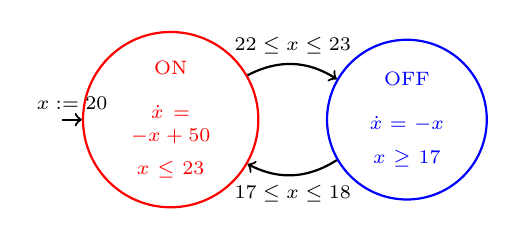
\begin{tikzpicture}[scale=0.6]
  \node[draw, circle, text width = 1.2cm, text centered, thick,color=red] (l1) at (0,0) {\scriptsize{ON\\ \ \\$\dot{x}=-x+50$\\ $x\leq 23$}};
  \node[draw, circle, text width = 1.2cm, text centered, color=blue, thick] (l2) at (5,0) {\scriptsize{OFF\\ \ \\$\dot{x}=-x$\\ $x\geq 17$}};
  \path[thick,->] (l1) edge[bend left] node[above] {\scriptsize{$22\leq x\leq 23$}} (l2);
  \path[thick,->] (l2) edge[bend left] node[below] {\scriptsize{$17\leq x\leq 18$}} (l1);
  \node (dummy) at (-2.5,0) {};
  \path[thick,->] (dummy) edge node[above] {\scriptsize{$x:=20$}} (l1);
 \end{tikzpicture}
\caption{On the left: the evolution of the temperature for the given thermostat initialized on the state (ON,$20$\textdegree C). On the right: the corresponding hybrid automata. Illustrations taken from Erika \'Abr\'aham's presentation in Genoa, Octorber 2015.}
\label{fig_thermostat}
\end{figure}

\label{exp_thermostat}
\end{example}

A hybrid automata is described by a set of possible discrete states and a set of continuous variables. The evolution of the variables is determined by the current discrete state. The current state of the system is defined by the discrete state it is in and by the current value of the continuous variables. A transition between two discrete states can be done under certain conditions (called a guard) over the variables, a well as staying in a given state (called the invariant of the state). A transition can reassign the variables.  



\begin{table}
\centering
\begin{tabular}{| c | c | c | c | c |}
	\hline	
	Sub- & derivative & conditions & bounded  & unbounded \\
	classes & & & reachability & reachability \\ \hline
	TA & $\dot x=1$ & $x\overset{?}{=}c$ & \textcolor{green}{\checkmark} &\textcolor{green}{\checkmark} \\ \hline
	& & $x\overset{?}{\in} [c_1;c_2]$ & &   \\	
   	IRA & $\dot x\in [c_1;c_2]$ & jump must reset &\textcolor{green}{\checkmark} &\textcolor{green}{\checkmark} \\ 
   	& & $x$ when $\dot x$ changes & &\\ \hline
   	RA & $\dot x\in [c_1;c_2]$ & $x\overset{?}{\in} [c_1;c_2]$ &\textcolor{green}{\checkmark} &\textcolor{red}{X} \\ \hline
   	LHA I & $\dot x=c$ & $x\overset{?}{=}g_{linear}$ &\textcolor{green}{\checkmark} &\textcolor{red}{X} \\ \hline
   	LHA II & $\dot x=f_{linear}$ & $x\overset{?}{=}g_{linear}$ &\textcolor{red}{X} &\textcolor{red}{X} \\ \hline
   	HA  & $\dot x=f$ & $\dot x=g$ &\textcolor{red}{X} &\textcolor{red}{X} \\ \hline
\end{tabular}
\label{tab_complexity}
\caption{Decidability results for subclasses of automata. $c$, $c_1$, $c_2$ are constants, $f$ and $g$ are function of other variables. TA~=~timed automata, IRA~=~ initialised rectangular automata, RA~=~rectangular automata, LHA I~=~hybrid automata with constant derivatives, LHA~II~=~hybrid automata with linear ODE's, HA~=~general hybrid automata.}
\end{table}

Analyse such systems is very difficult, the table~\ref{tab_complexity} gives the complexity of model checking for different classes of automata. Several methods exist to deal with this problem, theorem proving (model for a solver), interval based methods(model it for an SMT solver) and flowpipe computation. This paper contributes to the flowpipe-construction-based reachability analysis methods. 

As the model checking becomes rapidly non-decidable, the idea of the flowpipe computation is to determine an over approximation of a pipe containing the continuous variables at any instant. To do so, the time is discretized and, at each time step, all the possible values of the continuous variables are determined (analytically if the system is linear, with approximation otherwise). The successive sets containing the potential values of the variables are then linked together with bigger sets that includes all the possible values between the two instants. The result is a connected set containing all the possible values for the variables at any time. Figure~\ref{fowpipeconstruction} illustrate the construction of the "linking" phase of the flowpipe construction and an example of flowpipe fully constructed. The construction of the flowpipe stops at a given time limit or when a fix point is reached.

\begin{figure}
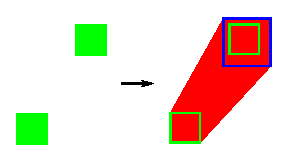
\includegraphics[scale=1.2]{images/flowpipe.eps}
missing
\caption{On the left: an example of the construction of a containing set for all the possible values between two sets obtained by analytic solving (in green). First bloat one of the sets(in blue), then take the convex hull of the resulting sets (in red). On the right: an example of fully constructed flowpipe.}
\label{fowpipeconstruction}
\end{figure}

There exists different sub-methods for the flowpipe construction, each corresponding to different methods to describe the sets of the possible values of the variables. Zonotopes, support functions and boxes are examples of representations. Several operations have to be performed on these sets along the way, for instance intersections to detect a collision with a forbidden state. How these set are described in the machine has a heavy influence on the cost to do one or another operation. The internship is about a method to switch between two representations of polyhedra: the $V$ representation and the $H$ representation according to Theorem~\ref{thm_representation}. First some notations and definitions for the rest of the paper:
 
\begin{definition}[Some geometry]
	The problem is studied in $\mathbb{R}^d$.
	\begin{itemize}
	\item $conv(V)$ defines the convex hull of the set of vertices $V$: $\{ x\in\mathbb{R}^d| x=\sum_{v\in V} \lambda_v v, \sum_{v\in V} \lambda_v =1, \forall v \in V, \ 0\leq \lambda_v \in \mathbb{R} \}$.
	\item $cone(C)$ defines the conic hull of the vectors in $C$: $\{ x\in\mathbb{R}^d| x=\sum_{c\in C} \lambda_c c, \forall c \in C,\ 0\leq \lambda_c \in \mathbb{R} \}$.
	\item $lineal(L)$ is the linear space generated by $L$: $\{ x\in\mathbb{R}^d| x=\sum_{l\in L} \lambda_l l, \forall l \in L,\ \lambda_c \in \mathbb{R} \}$. 
	\item In the paper, a sum between two sets is the Minkowsky sum: $S_1+S_2=\{s_1+s_2|s_1\in S_1,\ s_2 \in S_2 \}$.
	\item A half-space $h$ is an area of $\mathbb{R}^d$ defined by a normal vector $a$ and a constant $b$, $h=\{x\in\mathbb{R}^d|x.a\leq b\}$, its border is the hyperplane $\{x\in\mathbb{R}^d|x.a = b\}$. A family of half-spaces are said independent is their normal vectors are independent, and independent hyperplanes are defined respectively , $d$ independent hyperplanes intersect in a vertex.
	\item Let $A$ be a matrix which rows are normal vectors of a finite set of half-spaces and $B$ the column vector composed by the corresponding constants. $P(A,B)=\{x\in\mathbb{R}^d|Ax\leq B\}$ is the set of the points contained in all the half-spaces.
	\item An $H$-polyhedron $P$ is the intersection of a given finite set of half-spaces. There exist $A$ and $B$ such that $P=P(A,B)$.
	\item A $V$-polyhedron $P$ is the Minkowsky sum (from now on refereed as sum) of the convex hull of a finite set of points and a conic hull of a finite set of points, $P=conv(V)+cone(C)$ for some finite $V$ and $C$.
	\item A polyhedron is an $H$-polyhedron or a $V$-polyhedron.
	\item A polytope is a bounded polyhedron (and respectively with $H$ and $V$ polytopes).
	\end{itemize}
\end{definition}


\begin{theorem}[Polyhedra representation]
A Subset $P\subseteq\mathbb{R}^d$ is an $H$-polyhedron if and only if it is a $V$-polyhedron.
\label{thm_representation}
\end{theorem} 

\begin{figure}
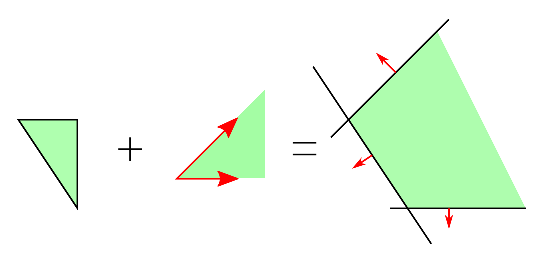
\includegraphics[scale=1]{images/poly.eps}
\caption{Illustration of Theorem~\ref{thm_representation}. From left to right: the sum of the convex hull of a set of vertices and a cone equals an intersection of half-spaces.}
\end{figure}

These two representations have their own advantages and disadvantages, which are summed up  in Tableau~\ref{comparison tab}, being able to switch between these two representations is thus crucial.

\begin{table}
\begin{tabular}{| c | c | c | c |}
	\hline	
				    & $.\ \cap\ .$ & $.\ \cup\ .$ & $.\ +\ .$ \\ \hline
	$V$-Polyhedra   & $-$ & $+$ & $+$ \\ \hline
   	$H$-Polyhedra   & $+$ & $-$ & $-$\\ \hline
\end{tabular}
\caption{Comparison of the cost of different operations between the two representation of the polyhedra.}
\label{comparison tab}
\end{table}

The hosting research group develops, in the context of the HyPro project, an open-source stand-alone C++ library for the most relevant geometric state set representations like covering boxes, polytopes, zonotopes, support functions... 
The library allows the combination of different representations and over-approximative conversion between them. So far it includes conversion between bounded $V$ and $H$-Polyhedra, the objective of the internship is to expand the library with the conversion between unbounded polyhedra.

The method developed in this paper and the library is an extension of a method for to convert $H$-polytopes into $V$-polytopes. This method was not the one implemented in HyPro, its implementation was part of the contribution too.

Section~\ref{section_sota} is a state of the art, presenting a method containing the main idea used in this paper: the simplex algorithm, and an algorithm used for the conversion of bounded $H$-polyhedra into $V$-polyhedra: Fukuda's algorithm. Section~\ref{section_contrib} is the contribution: how to use Fukuda's algorithm on unbounded $H$-polyhedra and how to reduce the conversion of unbounded $V$-polyhedra into $H$-polyhedra into the previously resolved problem. This reports ends by a summing up conclusion in Section~\ref{section_conclusion}. 



